% !TEX root = ../thesis.tex

\chapter{Training und Test der Machine-Learning-Klassifikatoren}
\label{training}

\paragraph{Ausblick:}
Dieses Kapitel gibt einen detaillierten Einblick in das Training und den Testprozess der Machine-Learning-Klassifikatoren. Dazu werden zunächst die Auswahl der verwendeten Werkzeuge und der Klassifikationsalgorithmen erläutert. Anschließend findet eine Analyse der Trainings- und Testprozesse der Klassifikatoren statt. Dies umfasst außerdem die Auflistung der finalen Konfigurationen der jeweiligen Klassifikatoren.
\\
\hrule

\section{Auswahl der Werkzeuge und der Klassifikationsalgorithmen}

Durch die Wahl der Programmiersprache Python war die Entscheidung zur Auswahl eines bestimmten Machine-Learning-Werkzeugs bereits absehbar. Zur Anwendung kommt die Python-Library scikit-learn\footnote{\href{https://scikit-learn.org/}{https://scikit-learn.org/}}, die im Jahr 2007 von Pedregosa et. al entwickelt wurde \cite{scikit}. Das Werkzeug bietet eine große Auswahl an Machine-Learning-Algorithmen für überwachtes und unüberwachtes Lernen und ermöglicht darüber hinaus eine einfache Verwendung sowie eine einfache Einbindung weiterer Python-Libraries, wie beispielsweise die Matplotlib zur Erstellung von mathematischen Darstellungen \cite{scikit}.

Ebenfalls wird der WEKA-Workbench\footnote{\href{https://www.cs.waikato.ac.nz/ml/weka/}{https://www.cs.waikato.ac.nz/ml/weka/}} als weiteres Machine-Learning-Wekzeug verwendet. Im Rahmen der strukturierten Literaturanalyse zu Beginn der Erarbeitung der Masterarbeit, erwies sich dieses Werkzeug durch zahlreiche Zitierungen in wissenschaftlichen Arbeiten (unter anderem in \cite{Hammouri2018,Queiroz2016,Ratzinger2008}) ebenfalls als geeignet für die zugrundeliegende Aufgabe. Der WEKA-Workbench (WEKA als Akronym für \textbf{W}aikato \textbf{E}nvironment for \textbf{K}nowledge \textbf{A}nalysis) wurde an der University of Waikato in Neuseeland entwickelt und bietet eine große Kollektion an Machine-Learning-Algorithmen und Preprocessing-Tools zur Verwendung innerhalb einer grafischen Benutzeroberfläche \cite{Weka2016}. Es existieren zudem Schnittstellen für die Programmiersprache Java \cite{Weka2016}. 

Die Verwendung von zwei Machine-Learning-Werkzeugen ermöglicht einen Vergleich der jeweiligen Implementierungen der verwendeten Klassifikationsalgorithmen in der anschließenden Evaluation. Eine Übersicht über die ausgewählten Klassifikationsalgorithmen je Werkzeug befindet sich in \autoref{tab:classifiers}. Kurze Erläuterungen der Algorithmen befinden sich im Anschluss.

\begin{table}
\centering
\caption{Zum Training verwendete Klassifikationsalgorithmen}
\label{tab:classifiers}
\resizebox{\linewidth}{!}{%
\begin{tabular}{|>{\hspace{0pt}}p{0.497\linewidth}|>{\hspace{0pt}}p{0.499\linewidth}|} 
\hline
\textbf{scikit-learn}  & \textbf{WEKA}  \\ 
\hline
Decision Trees & J48-Decision-Trees \\
k-Nearest-Neighbors & k-Nearest-Neighbors \\
Ridge Classifier & Logistic Regression \\
Na\"{\i}ve Bayes & Na\"{\i}ve Bayes \\
künstliche neuronale Netze & künstliche neuronale Netze \\
Random Forest & Random Forest \\
Stochastic Gradient Descent & Stochastic Gradient Descent \\
Support Vector Machines & Support Vector Machines \\
\hline
\end{tabular}
}
\end{table}

\label{algorithms}
\textbf{Decision Trees\medskip}\\
Decision Trees (deutsch: Entscheidungsbäume) zählen zu den meistverwendeten Klassifikatoren im Bereich des supervised Machine Learnings. Studien belegen, dass sie hinsichtlich der Verwendung im Kontext der Fehlererkennung die häufigste Anwendung finden \cite{Son2019}. Decision Trees sind gerichtete und verwurzelte Bäume, die als rekursive Partition der Eingabemenge des Datensets aufgebaut werden \cite{Rokach2005}. Den Ursprung des Baumes bildet die Wurzel, welche keine eingehenden Kanten besitzt - alle weiteren Knoten besitzen jedoch eine eingehende Kante \cite{Rokach2005}. Diese Knoten teilen wiederum die Eingabemenge anhand einer vorgegebenen Funktion in zwei oder mehr Unterräume der Menge auf \cite{Rokach2005}. Meist geschieht dies anhand eines Attributs, sodass die Eingabemenge anhand der Werte des einzelnen Attributs geteilt wird \cite{Rokach2005}. Die Blätter des Baumes bilden die Zielklassen ab. Eine Klassifizierung kann folglich durchgeführt werden, indem man von der Wurzel bis zu einem Blatt den Kanten anhand der entsprechenden Werte der Eingangsmenge folgt. Es existieren verschiedene Algorithmen zur Erstellung von Decision Trees. Bekannte Stellvertreter dieser sind ID3, C4.5 (J48) und CART \cite{Rokach2005}. Der grundlegende Aufbau eines Decision Trees ist in \autoref{fig:dt} dargestellt.

\begin{figure}[H]
    \centering
    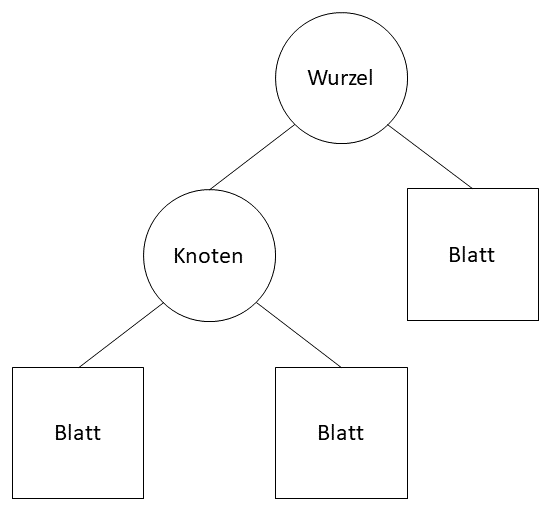
\includegraphics[width=0.5\textwidth]{images/DT}
    \caption{Grundsätzlicher Aufbau eines Decision Trees\label{fig:dt}}
\end{figure}

Eine Besonderheit von Decision Trees stellen sogenannte Random Forests dar. Diese beschreiben eine Lernmethode von Klassifikatoren, bei der mehrere einzelne Decision Trees gleichzeitig erzeugt werden und deren Ergebnisse anschließen aggregiert werden \cite{Alam2013}. Dazu erhält jeder Decision Tree eine Teilmenge der Eingabemenge des Datensets \cite{Alam2013}. Random Forests eigenen sich besonders zur Anwendung, wenn viele Attribute im Datenset vorhanden sind \cite{Alam2013}.

\textbf{k-Nearest-Neighbors\medskip}\\
Ein k-Nearest-Neighbor-Klassifikator (deutsch: k-nächste-Nachbarn) basiert auf zwei Konzepten \cite{Zhang2016}. Das erste Konzept basiert auf der Abstandsmessung zwischen den Werten der zu klassifizierenden Datenmenge und den Werten der Attribute des Datensets \cite{Zhang2016}. Die Abstandmessung erfolgt in der Regel durch die Berechnung der Euklidischen Distanz $D(p,q)$:

\[D(p,q)=\sqrt{\sum_1^n(p_{n}-q_{n})^{2}}\] 

Die Anzahl der Attribute wird durch den Parameter $n$ wiedergegeben, $p$ und $q$ repräsentieren jeweils die Werte der zu klassifizierenden Datenmenge und die Werte der Attribute des Datensets. Das zweite Konzept bildet der Parameter $k$, der angibt, wie viele nächste Nachbarn zum Vergleich der zuvor berechneten Abstände in Betracht gezogen werden \cite{Zhang2016}. Bei einem $k > 1$ wird diejenige Zielklasse gewählt, deren Auftreten innerhalb der nächsten Nachbarn überwiegt.

\textbf{Künstliche neuronale Netze\medskip}\\
Künstliche neuronale Netze (englisch: Artificial Neural Networks) verwenden nicht-lineare Funktionen zur schrittweisen Erzeugung von Beziehungen zwischen der Eingabemenge und den Zielklassen durch einen Lernprozess \cite{Linder2004}. Sie sind angelehnt an die Funktionsweise von biologischen Nervensystemen und bestehen aus einer Vielzahl von einander verbundenen Berechnungsknoten, den Neuronen \cite{OShea2015}. Der grundsätzliche Aufbau eines künstlichen neuronalen Netzes kann in \autoref{fig:ann} eingesehen werden. Der Lernprozess besteht aus zwei Phasen - einer Trainingphase und einer Recall-Phase \cite{Linder2004}. In der Trainingsphase werden die Eingabedaten, meist als multidimensionaler Vektor, in den Input-Layer geladen und anschließend an die Hidden-Layer verteilt \cite{OShea2015}. In den Hidden-Layers werden dann Entscheidungen anhand der Beziehungen zwischen den Eingabedaten und Zielklassen sowie die den Verbindungen zuvor zugewiesenen Gewichtsfaktoren getroffen \cite{Linder2004,OShea2015}. Im Rahmen der Recall-Pahse werden die wird die Vorhersage basierend auf der zu klassifizierenden Datenmenge anhand der zuvor getroffenen Entscheidungen der Hidden-Layers getroffen und an die jeweiligen Output-Layer, welche die Werte der Zielklasse repräsentieren, weitergeleitet\cite{Linder2004}. 

\begin{figure}[H]
    \centering
    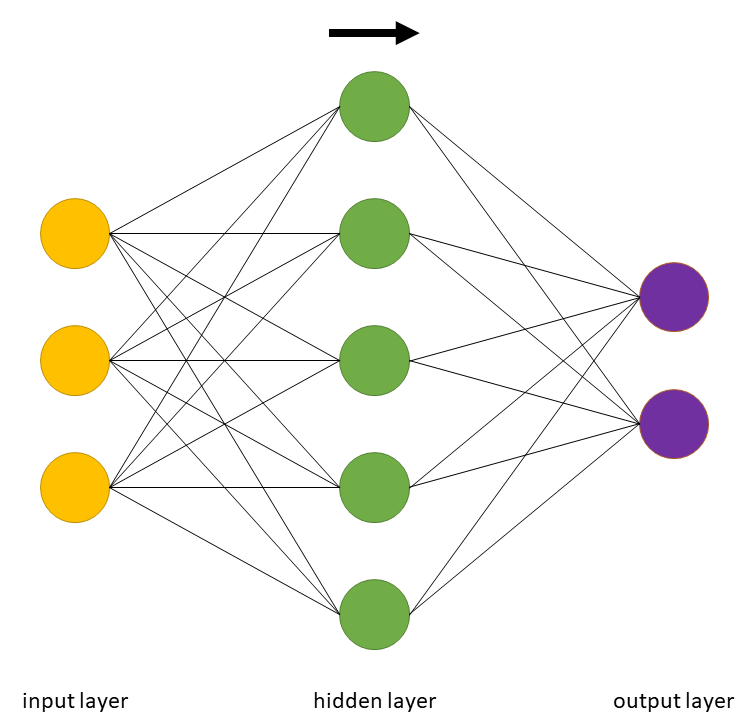
\includegraphics[width=0.5\textwidth]{images/ANN}
    \caption{Grundsätzlicher Aufbau eines KNN mit drei Input-Layer-Neuronen, fünf Hidden-Layer-Neuronen und zwei Output-Layer-Neuronen\label{fig:ann}}
\end{figure}

\textbf{Na\"{\i}ve Bayes\medskip}\\
Na\"{\i}ve-Bayes-Klassifikatoren zählen zu den linearen Klassifikatoren und basieren auf dem Satz von Bayes. Die Bezeichnung \glqq naiv\grqq{} erhält der Klassifikator durch die Annahme, dass die Attribute der Eingabemenge unabhängig voneinander sind \cite{Raschka2014}. Diese Annahme wird zwar in der realen Verwendung des Klassifikators häufig verletzt, dennoch erzielt er in der Regel eine hohe Performanz \cite{Raschka2014}. Der Klassifikator gilt als effizient, robust, schnell und einfach implementierbar \cite{Raschka2014}. Die zur Durchführung einer Klassifikation mittels Na\"{\i}ve Bayes benötigte Formel nach Thomas Bayes ist in \autoref{fig:nb} samt Erläuterung der einzelnen Faktoren aufgeführt.

\begin{figure}[H]
    \centering
    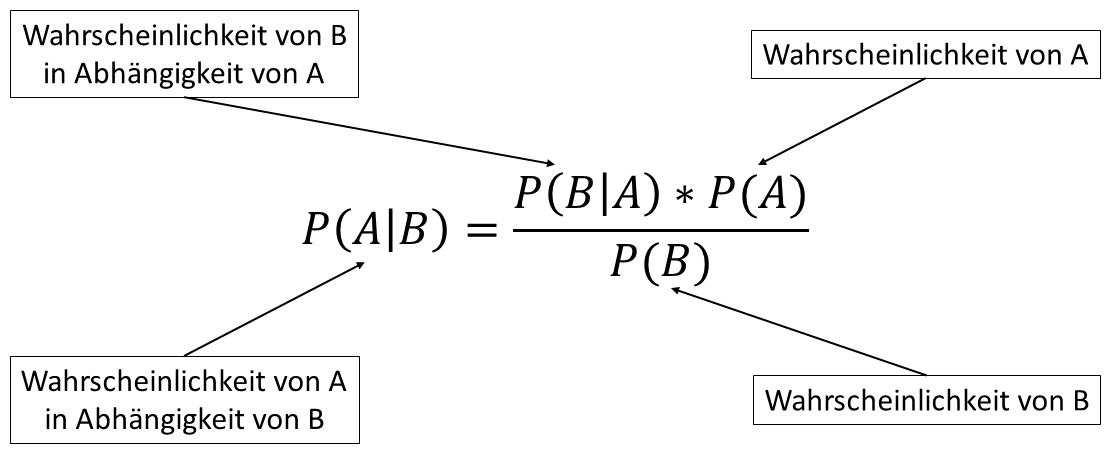
\includegraphics[width=0.6\textwidth]{images/NB}
    \caption{Satz von Bayes als Grundlage des Na\"{\i}ve-Bayes-Klassifikators\label{fig:nb}}
\end{figure}

Es existiert zudem eine Mehrzahl an Varianten des Na\"{\i}ve-Bayes-Klassifikators, die verschiedene Annahmen über die Verteilung der Attribute der Eingabemenge machen. Beispiele dafür sind der Gaußsche-Na\"{\i}ve-Bayes (normalverteilte Attribute), der multinomiale Na\"{\i}ve-Bayes (multinomiale Verteilung der Attribute) sowie der Bernoulli-Na\"{\i}ve-Bayes (unabhängige binäre Attribute).

\textbf{Logistische Regression\medskip}\\
Logistische-Regressions-Klassifikatoren (englisch: Logistic Regression) basieren auf dem mathematischen Konzept des Logits, welcher den natürlichen Logarithmus eines Chancenverhältnisses beschreibt \cite{Peng2002}. Seine Formel lautet:

\[logit(Y) = ln(\frac{\pi}{1-\pi})\]

$Y$ beschreibt dabei die zu klassifizierende Datenmenge, wohingegen $\pi$ die Verhältnisse der Wahrscheinlichkeiten der Werte der Attribute der Eingabemenge bezeichnet. Am besten geeignet ist dieser Klassifikator für eine Kombination aus kategorischen oder kontinuierlichen Eingabedaten und kategorischen Zielklassen \cite{Peng2002}. Der von scikit-learn zur Verfügung stehende Ridge Classifier basiert ebenfalls auf dem Konzept der logistischen Regression.

\textbf{Stochastic Gradient Descent\medskip}\\
Ein Stochastic-Gradient-Descent-Klassifikator basiert auf dem Gradientenverfahren (englisch: Gradient Descent), welches das Ziel hat, zu einem gegebenen $x$ das minimale $y$ zu finden \cite{Srinivasan2019}. Im Falle der Klassifikation mittels Machine Learning bezeichnet $x$ dabei die zu klassifizierende Eingabemenge und $y$ das erwartete Ergebnis der Klassifikation. Minimiert werden sollen dabei die \glqq Kosten\grqq{}, die sich aus der Ermittlung der Ergebnisse ergeben.

\textbf{Support Vector Machines\medskip}\\
Support Vector Machines verfolgen das Ziel, eine sogenannte \glqq Hyperplane\grqq{} in einem n-dimen-sionalen Raum (n = Anzahl der Attribute der Eingabemenge) zu finden, welche die Datenpunkte der Eingabemenge eindeutig klassifizieren kann \cite{Gandhi2018}. Die Hyperplane beschreibt eine Trennlinie beziehungsweise Trennfläche, mit deren Hilfe die Daten der zu klassifizierenden Menge den Zielklassen zuordnen lassen \cite{Luber2019}. Dabei gilt es, dass die Trennflächen, welche die Eingangsmenge anhand der Attribute in verschiedene Trennungsebenen unterteilen, einen möglichst großen Abstand ohne Datenpunkte voneinander haben \cite{Luber2019}. Dies funktioniert sowohl für linear als auch nicht-lineare trennbare Mengen.

Alle zuvor vorgestellten Klassifikationsalgorithmen sind bereits in den Werkzeugen scikit-learn und WEKA integriert. Sie erhalten als Eingabe das finale Datenset, dessen Erstellung im \hyperref[dataset]{vorherigen Kapitel} erläutert wurde. Die 13 berechneten Metriken bilden dabei die Attribute, wohingegen die Zielklasse durch die Label \glqq defekt\grqq{} und \glqq fehlerfrei\grqq{} abgebildet wird.

\fbox{\parbox{\linewidth}{\textsc{RQ2: WELCHE MACHINE-LEARNING-KLASSIFIKATOREN KOMMEN FÜR DIE GEGEBENE AUFGABE IN FRAGE?\medskip }\\
Es werden neun verschiedene Klassifikationsalgorithmen zur Anwendung kommen. Sieben Algorithmen werden sowohl mit scikit-learn als auch mit WEKA verwendet (DT / J48, KNN, NB, NN, RF, SGD, SVM). Jeweils ein Algorithmus ist werkzeugspezifisch (scikit-learn: RC, WEKA: LR), jedoch unterliegen beide Algorithmen dem Konzept der Regression. Das Hauptkriterium für die Auswahl sämtlicher Algorithmen war die vorherige Verwendung im Rahmen der wissenschaftlichen Literatur \cite{Son2019}.}}

\section{Analyse der Trainings- und Testprozesse}

Im weiteren Verlauf dieses Abschnitts und im Rahmen der Evaluation im folgenden Kapitel, werden die Namen der Klassifikatoren auf Abbildungen und in Tabellen abgekürzt. Die Abkürzungen können \autoref{tab:abbs} entnommen werden.

\begin{table}[H]
\centering
\caption{Zuordnung der verwendeten Abkürzungen}
\label{tab:abbs}
\resizebox{\linewidth}{!}{%
\begin{tabular}{|>{\centering\hspace{0pt}}p{0.15\linewidth}>{\hspace{0pt}}p{0.329\linewidth}|>{\centering\hspace{0pt}}p{0.15\linewidth}>{\hspace{0pt}}p{0.362\linewidth}|} 
\hline
\textbf{Abkürzung}  & \textbf{Klassifikator}  & \textbf{Abkürzung}  & \textbf{Klassifikator}  \\ 
\hline
DT / J48 & Decision Trees & RC & Ridge Classifier \\
KNN & k-Nearest-Neighbor & RF & Random Forest \\
LR & Logistic Regression & SGD & Stochastic Grandient Descent \\
NB & Na\"{\i}ve Bayes & SVM & Support Vector Machines \\
NN & künstliche neuronale Netze &  &  \\
\hline
\end{tabular}
}
\end{table}

Die Analyse des Trainingsprozesses zeigte, dass das dateibasierte Datenset stark unbalanciert hinsichtlich der Zielklasse ist. Mit einem Wert von etwa 98\% existieren weitaus mehr Einträge, die dem Label \glqq fehlerfrei\grqq{} zugeordnet sind. Balanciertheit, also ein ausgeglichenes Verhältnis (50:50 ist im binären Fall nicht zwingend notwendig) innerhalb der Zielklassen, ist jedoch eine Voraussetzung für das korrekte Erlernen der meisten Klassifikatoren. Eine Nichtbeachtung dieses Problem kann zu einer irreführenden Accuracy (Treffergenauigkeit des Klassifikators) führen, da die meisten Datensätze korrekt der überrepräsentierten Klasse zugeordnet werden. Als Lösung dieses Problems wurde der sogenannte SMOTE-Algorithmus auf das dateibasierte Datenset angewendet \cite{Chawla2002}. Der Algorithmus, dessen Akronym für \textbf{S}ynthetic \textbf{M}inority \textbf{O}ver-sampling \textbf{Te}chnique steht, führt ein Oversampling der unterrepräsentierten Klasse durch \cite{Chawla2002}. Anhand von nächste-Nachbarn-Berechnungen auf Basis der Euklidischen Distanz zwischen den Attributwerten der einzelnen Datensätze des Datensets, werden neue synthetische Datensätze hinzugefügt (Oversampling), sodass sich die Anzahl der Datensätze der relevanten Klasse erhöht \cite{Chawla2002}. Im hier durchgeführten Fall wurde der Prozentsatz für die Generierung der synthetischen Datensätze auf 3000 festgelegt, sodass für jeden vorhandenen Datensatz der unterrepräsentierten Klasse 30 zusätzliche synthetische Datensätze erzeugt wurden. So konnte der Anteil der Datensätze mit dem Label \glqq fehlerhaft\grqq{} auf etwa 27\% erhöht werden. In \autoref{fig:smoted} ist dargestellt, welchen Einfluss die Anwendung des SMOTE-Algorithmus auf die Accuracies der Klassifikatoren des datenbasierten Datensets im Rahmen des Testprozesses hatte. Das mit \glqq vorher\grqq{} deklarierte Diagramm zeigt, dass nahezu alle Klassifikatoren eine Accuracy von nahezu 100\% besitzen, was das zuvor beschriebene Problem widerspiegelt und eine unrealistische Situation darstellt. Das Diagramm, welches die Testergebnisse nach Anwendung des SMOTE-Algorithmus darstellt, weist hingegen wesentlich glaubwürdigere Accuracies auf.


\begin{figure}[]
    \centering
    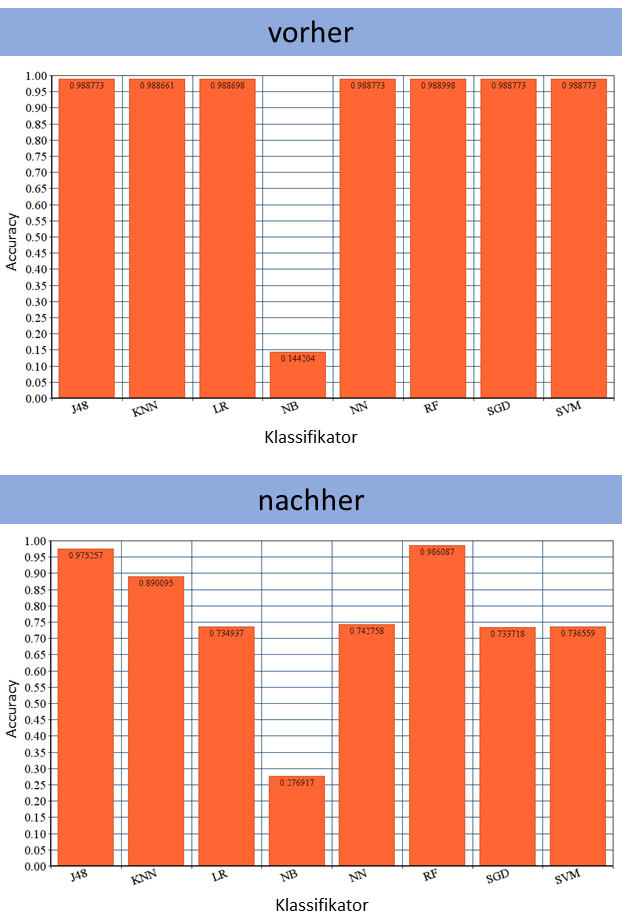
\includegraphics[width=0.8\textwidth]{images/smoted}
    \caption{Vergleich der Accuracies je Klassifikator vor und nach der Anwendung des SMOTE-Algorithmus auf das dateibasierte Datenset\label{fig:smoted}}
\end{figure}

Der Testprozess diente zur Erarbeitung der korrekten Konfiguration der Klassifikatoren. Dazu zählen das Festlegen von möglichen Parametern, die die Klassifikationsalgorithmen beeinflussen können, das Festlegen des optimalen Verhältnisses zwischen Training- und Testdatenset (Split-Ratio) sowie die Auswahl der effektivsten Kombination der gegebenen elf Attribute. In \autoref{fig:vergl1} ist zunächst dargestellt, welche Accuracies die jeweiligen Klassifikatoren pro Werkzeug und Datenset ohne eine angewendete Konfiguration erreichen. Gemessen wurden jeweils die Accuracies der Klassifikatoren für die Split-Ratios 85:15 (Training : Test), 80:20, 75:25, 70:30 und 65:35. Außerdem wurde für das Werkzeug WEKA die alternative Option zur Durchführung einer \glqq 10-fold-cross-validation\grqq{} berücksichtigt. Bei dieser Variante wird das Datenset in zehn gleich große Datensets aufgeteilt, welche dann jeweils mit einer Split-Ratio von 90:10 zur Anlernung eines Klassifikators dienen \cite{IanWitten}. Die Accuracy dieses Vorgangs wird anschließend als Durchschnitt der Accuracies der 10 Klassifikatoren gewertet \cite{IanWitten}. Die erwähnte Abbildung zeigt pro Klassifikator die höchste Accuracy die mithilfe der fünf Split-Ratios oder mithilfe der 10-fold-cross-validation gemessen werden konnte. 

\begin{figure}[]
    \centering
    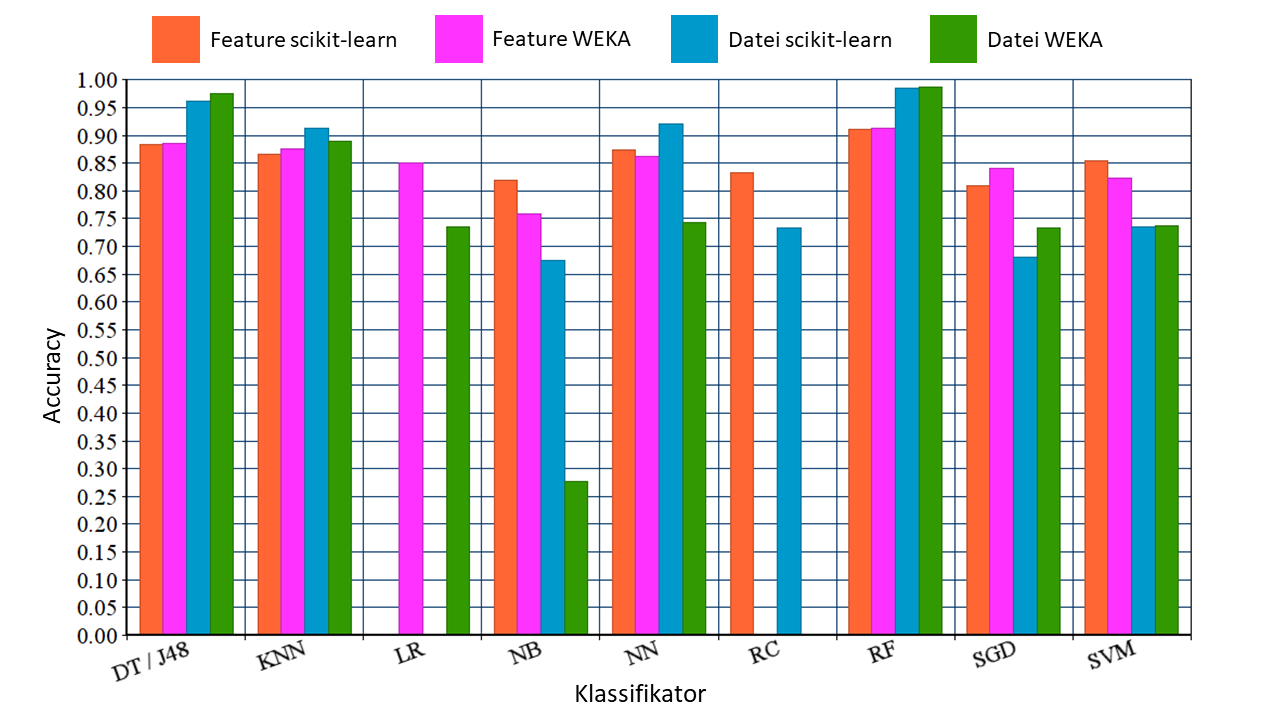
\includegraphics[width=\textwidth]{images/Vergleich1}
    \caption{Vergleich der Klassifikatoren und Werkzeuge im Hinblick auf ihre Accuracies\label{fig:vergl1}}
\end{figure}

Zur Auswahl der effektivsten Kombination der Attribute je Klassifikator wurde auf die von scikit-learn und WEKA bereitgestellten Werkzeuge zurückgegriffen. Sowohl scikit-learn als auch WEKA konnten nicht für jeden Klassifikator der beiden Datensets Kombinationen ausgeben. Dies bedingt entweder die Funktionsweise des Klassifikationsalgorithmus, die fehlende Unterstützung der Werkzeuge für einen bestimmten Klassifikator oder eine endlose Durchführung der Ermittlung der Kombination. Eine Übersicht der Konfiguration je Klassifikator des featurebasierten Datensets ist in \autoref{tab:configs_feat} dargestellt. Die Übersicht für das dateibasierte Datenset befindet sich in \autoref{tab:configs_file}.

\begin{table}
\centering
\caption{Übersicht der Konfigurationen des featurebasierten Datensets}
\label{tab:configs_feat}
\resizebox{\linewidth}{!}{%
\begin{tabular}{|c|l|l|} 
\hline
\textbf{Klassifikator}  & \multicolumn{1}{c|}{\textbf{Konfiguration scikit-learn} }                                                                                                                                                                           & \multicolumn{1}{c|}{\textbf{Konfiguration WEKA} }                                                                                                                                                     \\ 
\hline
DT / J48                & \begin{tabular}[c]{@{}l@{}}\begin{tabular}{@{\labelitemi\hspace{\dimexpr\labelsep+0.5\tabcolsep}}l}max\_features = \glqq sqrt\grqq\\Split-Ratio: 80:20\\Features: alle außer ADEV, DDEV \end{tabular}\end{tabular}                            & \begin{tabular}[c]{@{}l@{}}\begin{tabular}{@{\labelitemi\hspace{\dimexpr\labelsep+0.5\tabcolsep}}l}Split-Ratio: 10-x-v\\Features: alle außer DDEV, OEXP, \\MODD, NLOC \end{tabular}\end{tabular}        \\ 
\hline
KNN                     & \begin{tabular}[c]{@{}l@{}}\begin{tabular}{@{\labelitemi\hspace{\dimexpr\labelsep+0.5\tabcolsep}}l}k = 2\\Split-Ratio: 75:25 \end{tabular}\end{tabular}                                                                             & \begin{tabular}[c]{@{}l@{}}\begin{tabular}{@{\labelitemi\hspace{\dimexpr\labelsep+0.5\tabcolsep}}l}k = 1\\Split-Ratio: 10-x-v \end{tabular}\end{tabular}                                              \\ 
\hline
LR                      &                                                                                                                                                                                                                                     & \begin{tabular}{@{\labelitemi\hspace{\dimexpr\labelsep+0.5\tabcolsep}}l}Split-Ratio: 70:30 \end{tabular}                                                                                              \\ 
\hline
NB                      & \begin{tabular}[c]{@{}l@{}}\begin{tabular}{@{\labelitemi\hspace{\dimexpr\labelsep+0.5\tabcolsep}}l}Multinomial-NB\\Split-Ratio: 75:25 \end{tabular}\end{tabular}                                                                    & \begin{tabular}[c]{@{}l@{}}\begin{tabular}{@{\labelitemi\hspace{\dimexpr\labelsep+0.5\tabcolsep}}l}Split-Ratio: 10-x-v\\Features: COMM, EXP, MODD, ADDL \end{tabular}\end{tabular}                    \\ 
\hline
NN                      & \begin{tabular}[c]{@{}l@{}}\begin{tabular}{@{\labelitemi\hspace{\dimexpr\labelsep+0.5\tabcolsep}}l}hidden\_layer\_sizes = (13,13,13)\\max\_iter = 500\\Split-Ratio: 70:30 \end{tabular}\end{tabular}                                   & \begin{tabular}[c]{@{}l@{}}\begin{tabular}{@{\labelitemi\hspace{\dimexpr\labelsep+0.5\tabcolsep}}l}Hidden-Layer = (13,13,13)\\Split-Ratio: 85:15 \end{tabular}\end{tabular}                           \\ 
\hline
RC                      & \begin{tabular}[c]{@{}l@{}}\begin{tabular}{@{\labelitemi\hspace{\dimexpr\labelsep+0.5\tabcolsep}}l}StandardScaler\\Split-Ratio: 75:25\\Features: alle außer EXP, CYCO \end{tabular}\end{tabular}                                    &                                                                                                                                                                                                       \\ 
\hline
RF                      & \begin{tabular}[c]{@{}l@{}}\begin{tabular}{@{\labelitemi\hspace{\dimexpr\labelsep+0.5\tabcolsep}}l}n\_estimators = 200\\max\_features = \glqq sqrt\grqq\\Split-Ratio: 80:20\\Features: alle außer DDEV, MODD, REML \end{tabular}\end{tabular}  & \begin{tabular}[c]{@{}l@{}}\begin{tabular}{@{\labelitemi\hspace{\dimexpr\labelsep+0.5\tabcolsep}}l}Iterationen: 200\\Split-Ratio: 10-x-v\\Features: alle außer DDEV, OEXP \end{tabular}\end{tabular}  \\ 
\hline
SGD                     & \begin{tabular}[c]{@{}l@{}}\begin{tabular}{@{\labelitemi\hspace{\dimexpr\labelsep+0.5\tabcolsep}}l}loss = \glqq log\grqq\\penality = \glqq elasticnet\grqq\\Split-Ratio: 85:15\\Features: EXP, OEXP \end{tabular}\end{tabular}                        & \begin{tabular}[c]{@{}l@{}}\begin{tabular}{@{\labelitemi\hspace{\dimexpr\labelsep+0.5\tabcolsep}}l}Split-Ratio: 70:30\\Features: alle außer REML \end{tabular}\end{tabular}                           \\ 
\hline
SVM                     & \begin{tabular}[c]{@{}l@{}}\begin{tabular}{@{\labelitemi\hspace{\dimexpr\labelsep+0.5\tabcolsep}}l}LinearSVC\\max\_iter = 20000\\StandardScaler\\Split-Ratio: 75:25\\Features: alle außer DDEV, EXP, REML \end{tabular}\end{tabular} & \begin{tabular}[c]{@{}l@{}}\begin{tabular}{@{\labelitemi\hspace{\dimexpr\labelsep+0.5\tabcolsep}}l}Split-Ratio: 70:30\\Features: alle außer REML \end{tabular}\end{tabular}                           \\
\hline
\end{tabular}
}
\end{table}

\begin{table}
\centering
\caption{Übersicht der Konfigurationen des dateibasierten Datensets}
\label{tab:configs_file}
\resizebox{\linewidth}{!}{%
\begin{tabular}{|c|l|l|} 
\hline
\textbf{Klassifikator}  & \multicolumn{1}{c|}{\textbf{Konfiguration scikit-learn} }                                                                                                                                                                   & \multicolumn{1}{c|}{\textbf{Konfiguration WEKA} }                                                                                                                            \\ 
\hline
DT / J48                & \begin{tabular}[c]{@{}l@{}}\begin{tabular}{@{\labelitemi\hspace{\dimexpr\labelsep+0.5\tabcolsep}}l}max\_features = \glqq sqrt\grqq\\Split-Ratio: 85:15\\Features: DDEV, EXP \end{tabular}\end{tabular}                                & \begin{tabular}{@{\labelitemi\hspace{\dimexpr\labelsep+0.5\tabcolsep}}l}Split-Ratio: 10-x-v \end{tabular}                                                                    \\ 
\hline
KNN                     & \begin{tabular}[c]{@{}l@{}}\begin{tabular}{@{\labelitemi\hspace{\dimexpr\labelsep+0.5\tabcolsep}}l}k = 1\\Split-Ratio: 75:25 \end{tabular}\end{tabular}                                                                     & \begin{tabular}[c]{@{}l@{}}\begin{tabular}{@{\labelitemi\hspace{\dimexpr\labelsep+0.5\tabcolsep}}l}k = 10\\Split-Ratio: 10-x-v \end{tabular}\end{tabular}                    \\ 
\hline
LR                      &                                                                                                                                                                                                                             & \begin{tabular}{@{\labelitemi\hspace{\dimexpr\labelsep+0.5\tabcolsep}}l}Split-Ratio: 85:15 \end{tabular}                                                                     \\ 
\hline
NB                      & \begin{tabular}[c]{@{}l@{}}\begin{tabular}{@{\labelitemi\hspace{\dimexpr\labelsep+0.5\tabcolsep}}l}Bernoulli-NB\\Split-Ratio: 75:25 \end{tabular}\end{tabular}                                                              & \begin{tabular}[c]{@{}l@{}}\begin{tabular}{@{\labelitemi\hspace{\dimexpr\labelsep+0.5\tabcolsep}}l}Split-Ratio: 70:30\\Features: MODS, CYCO \end{tabular}\end{tabular}       \\ 
\hline
NN                      & \begin{tabular}[c]{@{}l@{}}\begin{tabular}{@{\labelitemi\hspace{\dimexpr\labelsep+0.5\tabcolsep}}l}hidden\_layer\_sizes = (13,13,13)\\max\_iter = 500\\Split-Ratio: 80:20 \end{tabular}\end{tabular}                            & \begin{tabular}[c]{@{}l@{}}\begin{tabular}{@{\labelitemi\hspace{\dimexpr\labelsep+0.5\tabcolsep}}l}Hidden-Layer = (13,13,13)\\Split-Ratio: 75:25 \end{tabular}\end{tabular}  \\ 
\hline
RC                      & \begin{tabular}[c]{@{}l@{}}\begin{tabular}{@{\labelitemi\hspace{\dimexpr\labelsep+0.5\tabcolsep}}l}StandardScaler\\Split-Ratio: 85:15\\Features: alle außer DDEV \end{tabular}\end{tabular}                                 &                                                                                                                                                                              \\ 
\hline
RF                      & \begin{tabular}[c]{@{}l@{}}\begin{tabular}{@{\labelitemi\hspace{\dimexpr\labelsep+0.5\tabcolsep}}l}n\_estimators = 200\\max\_features = \glqq sqrt\grqq\\Split-Ratio: 85:15\\Features: alle außer EXP, OEXP \end{tabular}\end{tabular} & \begin{tabular}[c]{@{}l@{}}\begin{tabular}{@{\labelitemi\hspace{\dimexpr\labelsep+0.5\tabcolsep}}l}Iterationen: 200\\Split-Ratio: 85:15 \end{tabular}\end{tabular}           \\ 
\hline
SGD                     & \begin{tabular}[c]{@{}l@{}}\begin{tabular}{@{\labelitemi\hspace{\dimexpr\labelsep+0.5\tabcolsep}}l}loss = \glqq log\grqq\\penality = \glqq elasticnet\grqq\\Split-Ratio: 80:20\\Features: ADDL \end{tabular}\end{tabular}                     & \begin{tabular}{@{\labelitemi\hspace{\dimexpr\labelsep+0.5\tabcolsep}}l}Split-Ratio: 85:15 \end{tabular}                                                                     \\ 
\hline
SVM                     & \begin{tabular}[c]{@{}l@{}}\begin{tabular}{@{\labelitemi\hspace{\dimexpr\labelsep+0.5\tabcolsep}}l}LinearSVC\\max\_iter = 20000\\StandardScaler\\Split-Ratio: 75:25 \end{tabular}\end{tabular}                               & \begin{tabular}{@{\labelitemi\hspace{\dimexpr\labelsep+0.5\tabcolsep}}l}Split-Ratio: 85:15 \end{tabular}                                                                     \\
\hline
\end{tabular}
}
\end{table}

Mithilfe der Konfigurationen konnten die finalen Klassifikatoren erzeugt werden, welche als Grundlage für die Evaluation und den gegenseitigen Vergleich innerhalb und zwischen dem featurebasierten und dem dateibasierten Datenset dienen. Die Evaluation erfolgt im \hyperref[evaluation]{folgenden Kapitel}.

\cleardoublepage